\documentclass[portrait]{sciposter}

\usepackage{amsmath}
\usepackage{amssymb}
\usepackage{multicol}
\usepackage{graphicx}
\usepackage{enumerate}
\usepackage[english]{babel}
\usepackage{fancyvrb}   % for the Verbatim environment
%\usepackage{fancybullets}
%\usepackage{other packages you may want to use}

\usepackage{amsthm}
\usepackage{tikz}
\usepackage{booktabs}
\usepackage{url}

\usepackage{tabularx}
\newcolumntype{R}{>{\raggedleft\arraybackslash}X}

\definecolor{BoxCol}{RGB}{102,153,255}
% uncomment for grey background to \section boxes 
% for use with default option boxedsections

%\definecolor{BoxCol}{rgb}{0.9,0.9,1}
% uncomment for light blue background to \section boxes 
% for use with default option boxedsections

%\definecolor{SectionCol}{rgb}{0,0,0.5}
% uncomment for dark blue \section text 

\newcommand{\bigO}{\mathcal{O}}

\title{\begin{Huge}
A$^*$mbush family: A$^*$ Variations for Ambush 
Behavior and Path Diversity Generation
\end{Huge}}

% Note: only give author names, not institute
\author{Kelwin Fern\'andez, Glebys Gonz\'alez and Carolina Chang}
 
% insert correct institute name
                    
\institute{Universidad Sim\'on Bol\'ivar.
           Caracas, Venezuela}

%\email{kelwin@gia.usb.ve}  % shows author email address below institute

%\date is unused by the current \maketitle

% The following commands can be used to alter the default logo settings
%\leftlogo[0.9]{chenille}{  % defines logo to left of title (with scale factor)
%\rightlogo[0.52]{otherlogo}  % same but on right
% NOTE: the logo image files chenille.png, resp. otherlogo.png must be 
%       present in the same directory as this LaTeX source, either
%       in the .png format, or in any other supported format
%%%%%%%%%%%%%%%%%%%%%%%%%%%%%%%%%%%%%%%%%%%%%%%%%%%%%%%%%%%%%%%%%%%%%%%%%%

\begin{document}
%*** print the poster header defined above: title, authors, affiliations:
\maketitle

%*** facultative: where the poster was presented (appears as a left footer):
\conference{Motion in Games, Rennes, France, November, 2012}

\begin{multicols}{2}
\section*{\large{Motivation}}
\begin{large}
\begin{itemize}
\item Generating agents with \textbf{intelligent-looking} behaviors
has been a constant challenge in the area of Artificial
Intelligence for video games. The user expects to see
agents that can perform \textbf{tactical movements} and
\textbf{group strategies}.

%\item These behaviors tend to be complex in their implementation
%and usually result in pre-established moves that can be easily
%identified by the user.

\item 
A situation that appears frecuently in this area 
is having a group of agennts trying to reach 
 a common target  through pathfinding.
The goal point is usually given by a location in the game map
(potentially the opponent's position).

\item A well known approach is to generate the \textbf{minimal path}
towards the objective.
When the algorithm is executed independently by multiple agents,
it is very likely for the paths to be \textbf{confluent}. Thus,
route diversity and map exploration is prevented.

\includegraphics[width=0.15\textwidth, height=10cm]{figures/fps.jpg}
\includegraphics[width=0.15\textwidth, height=10cm]{figures/pacman.jpg}
\includegraphics[width=0.15\textwidth, height=10cm]{figures/do.png}

\bigskip
\item When the minimal path strategy is applied for chasing
the enemy, many escape paths are left open. Therefore,
it is of special interest to generate mechanisms of \textbf{route
diversification} that can produce ambush behaviors.
\end{itemize}
\end{large}

\end{multicols}

\section*{A$^*$mbush: The Initial Variation}

\begin{multicols}{3}
\section{Definici\'on Formal del Problema}
\label{sec:definition}

Sea $G = (V,E)$ un grafo (dirigido o no), donde $V$ es el conjunto de
nodos y $E$ el conjunto de arcos. Sea $A$ un conjunto de agentes
interesados en alcanzar un punto com\'un $t \in V$. Se tiene
que cada agente $a \in A$, se encuentra en algún nodo del grafo
denotado $pos(a)$. Además, se define para $a$ la función
de costos de su desplazamiento por el grafo
$\lambda_a : E \longrightarrow \mathbb{R}^{\geq 0}$.
Se considera, sin pérdida de generalidad, que $V$ y $E$ son comunes para
todos los agentes, con el fin de no generar inconsistencias en la
información compartida entre estos. Sin embargo, cada agente puede tener
función de costos distintas, adaptadas a sus restricciones.
Sea $path(a)$ con $a \in A$, el camino que está siguiendo el agente
$a$ hasta el nodo $t$.

Previamente, el grado de emboscada (\ref{eq:prev})
efectuado por el conjunto de agentes
$A$ al nodo $t$ se defini\'o como \cite{FGC12e}\cite{FGC12}:

\begin{small}
\begin{eqnarray}
 \Phi(t) &=& 
 \dfrac{|\{ i : path(j) = <pos(j),\ \ldots,\ i,\ t>, j \in A\}|}
	  {\min(|\{ <i,t> : <i,t> \in E \} |,|A|) }
\label{eq:prev}
\end{eqnarray}
\end{small}

Esta m\'etrica define la emboscada como la proporción de nodos adyacentes
al nodo objetivo desde los cuales algún agente está alcanzándolo. Normalizando
este valor con res\-pec\-to al m\'aximo n\'umero de nodos adyacentes a $t$ mediante
los cuales, con el n\'umero de agentes disponibles, podr\'ia \'este ser alcanzado.
Por lo tanto, $0 \leq \Phi(t) \leq 1$. Bajo estas condiciones, el objetivo
de un algoritmo de generaci\'on de emboscadas es maximilar el
valor de $\Phi(t)$, dando prioridad a la diversidad de los caminos
considerados por el conjunto de agentes sobre su optimalidad.

En la figura \ref{fig:prev_phi}, se pueden observar en el grafo
superior dos agentes situados en los nodos izquierdos. Los caminos
seleccionados por los agentes hasta el destino $t$ se presenta con
una l\'inea continua, mientras que los arcos no seleccionados se
presentan con una l\'inea segmentada. El n\'umero de nodos adyacentes
al destino es de cuatro. De estos cuatro nodos, s\'olo dos están siendo
considerados en los caminos de los agentes. Sin embargo, es el m\'aximo
grado de emboscada alcanzable con el n\'umero de agentes implicados.
En el escenario inferior se est\'an utilizando dos agentes para cubrir
una \'unica escapatoria, por lo que la emboscada no es \'optima.

\begin{figure}[htb]
	\begin{center}
		\begin{minipage}[b]{0.9\linewidth}
			\centering
			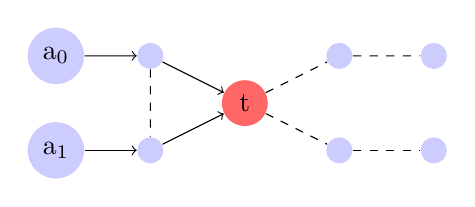
\begin{tikzpicture}
			  [scale=.6,auto=left,every node/.style={circle,fill=blue!20}]
			  \node (n1) at (1,3) {a$_0$};
			  \node (n2) at (3,3) { };
			  
	  		  \node (n3) at (1,1) {a$_1$};
			  \node (n4) at (3,1) { };
			  
			  \node[style={circle,fill=red!60}] (n5) at (5,2) {t};
			  
			  \node (n6) at (7,3) { };
			  \node (n7) at (7,1) { };
			  \node (n8) at (9,3) { };
			  \node (n9) at (9,1) { };
			  		  
			  \foreach \from/\to in {n1/n2,n2/n5,n3/n4,n4/n5}
			  \draw (\from) edge[->] (\to);
	
			  \foreach \from/\to in {n5/n6,n5/n7,n6/n8,n7/n9,n2/n4}
			  \draw (\from) edge[-,dashed] (\to);		  
			\end{tikzpicture}
			
			(a)\\
		\end{minipage}
		
		\bigskip
		\begin{minipage}[b]{0.9\linewidth}
			\centering
			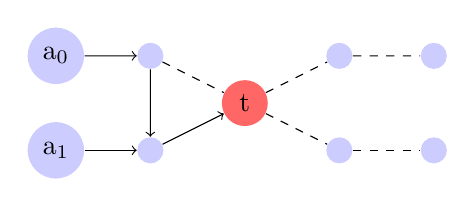
\begin{tikzpicture}
			  [scale=.6,auto=left,every node/.style={circle,fill=blue!20}]
			  \node (n1) at (1,3) {a$_0$};
			  \node (n2) at (3,3) { };
			  
	  		  \node (n3) at (1,1) {a$_1$};
			  \node (n4) at (3,1) { };
			  
			  \node[style={circle,fill=red!60}] (n5) at (5,2) {t};
			  
			  \node (n6) at (7,3) { };
			  \node (n7) at (7,1) { };
			  \node (n8) at (9,3) { };
			  \node (n9) at (9,1) { };
			  		  
			  \foreach \from/\to in {n1/n2,n3/n4,n4/n5,n2/n4}
			  \draw (\from) edge[->] (\to);
	
			  \foreach \from/\to in {n5/n6,n5/n7,n6/n8,n7/n9,n2/n5}
			  \draw (\from) edge[-,dashed] (\to);		  
			\end{tikzpicture}
			
			(b)\\
		\end{minipage}
	\end{center}
	\caption{\label{fig:prev_phi}
	     Ejemplos de emboscadas con dos agentes con valores de $\Phi$ de
	     $1.0$ para (a) dado que cubre dos caminos y $0.5$ para (b) dado que
	     cubre un camino. En el caso (b), se considera apenas un predecesor
	     del nodo $t$ de los dos predecesores posibles.
	}
\end{figure}

Sin embargo, esta m\'etrica penaliza casos donde no es posible alcanzar
una mejor emboscada, a\'un cuando se cuenta con suficientes agentes, debido
a la configuraci\'on del grafo y de las posiciones iniciales de estos. 
Ejemplos de estos casos pueden ser observados en la figura \ref{fig:error_phi}. En
la situaci\'on superior, se observa que a pesar de contar con cuatro agentes,
las dos salidas restantes no son alcanzables por estos sin pasar antes por el
nodo objetivo. Por otra parte, en la situaci\'on inferior, a pesar de que todas
las salidas son alcanzables por los agentes, no es posible alcanzar una
configuraci\'on de caminos capaz de cubrir todas las salidas. Para ambos
casos, a pesar de que la asignaci\'on de caminos es la mejor dadas las
condiciones iniciales, la m\'etrica originalmente planteada reporta resultados
sub\'optimos.

\begin{figure}[htb]
	\begin{center}
		\begin{minipage}[b]{0.9\linewidth}
			\centering
			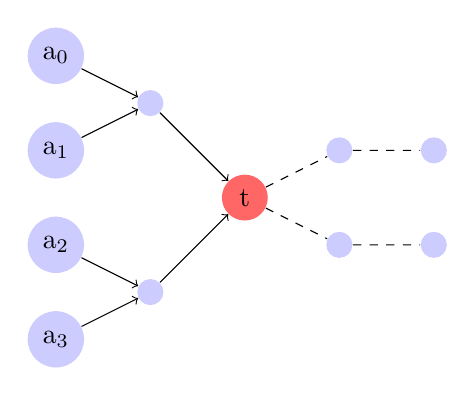
\begin{tikzpicture}
			  [scale=.6,auto=left,every node/.style={circle,fill=blue!20}]
			  \node (n11) at (1,7) {a$_0$};
			  \node (n12) at (1,5) {a$_1$};
			  \node (n2) at (3,6) { };
			  
	  		  \node (n31) at (1,3) {a$_2$};
	  		  \node (n32) at (1,1) {a$_3$};
			  \node (n4) at (3,2) { };
			  
			  \node[style={circle,fill=red!60}] (n5) at (5,4) {t};
			  
			  \node (n6) at (7,5) { };
			  \node (n7) at (7,3) { };
			  \node (n8) at (9,5) { };
			  \node (n9) at (9,3) { };
			  
			  \foreach \from/\to in {n11/n2,n12/n2,n2/n5,n31/n4,n32/n4,n4/n5}
			  \draw (\from) edge[->] (\to);
	
			  \foreach \from/\to in {n5/n6,n5/n7,n6/n8,n7/n9}
			  \draw (\from) edge[-,dashed] (\to);		  
			\end{tikzpicture}
			
			(a)\\
		\end{minipage}
		
		\bigskip
		\begin{minipage}[b]{0.9\linewidth}
			\centering
			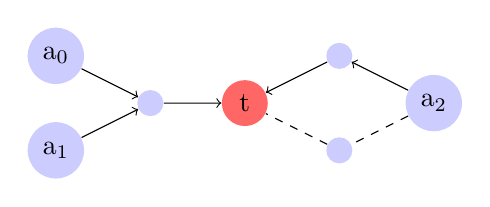
\begin{tikzpicture}
			  [scale=.6,auto=left,every node/.style={circle,fill=blue!20}]
			  \node (n11) at (1,3) {a$_0$};
			  \node (n12) at (1,1) {a$_1$};
			  \node (n2) at (3,2) { };
			  
	  		  \node (n3) at (9,2) {a$_2$};
			  \node (n41) at (7,3) { };
  			  \node (n42) at (7,1) { };
  			  
			  \node[style={circle,fill=red!60}] (n5) at (5,2) {t};
			  
			  \foreach \from/\to in {n11/n2,n12/n2,n2/n5,n3/n41,n41/n5}
			  \draw (\from) edge[->] (\to);
	
			  \foreach \from/\to in {n3/n42,n42/n5}
			  \draw (\from) edge[-,dashed] (\to);		  
			\end{tikzpicture}
			
			(b)
		\end{minipage}
	\end{center}
	\caption{\label{fig:error_phi}
	     Casos en los cuales la m\'etrica original pe\-na\-li\-za emboscadas
	     \'optimas. (a) Caso de no alcanzabilidad. (b) Caso de no existencia
	     de mejor asignaci\'on posible.}
\end{figure}

Por lo tanto, es necesario utilizar una nueva medida de emboscada
para poder discriminar correctamente entre las escapatorias que podr\'ian
ser cubiertas por alg\'un agente y aquellas que no. Esta nueva medida,
denotada por $\Phi^*$ (\ref{eq:new}) busca normalizar a los agentes utilizando
el tamaño de la m\'axima asociaci\'on de agentes a los nodos predecesores
del objetivo que \'estos son capaces de alcanzar. Se define $\Phi^*$ como:

\begin{small}
\begin{eqnarray}
 \Phi(t) &=& 
\dfrac{|\{ i : path(j) = <pos(j),\ \ldots,\ i,\ t>, j \in A\}|}
	  {|\{ y : (x,y) \in MaxMatching(BipG(G,A,t))\}|}
\label{eq:new}
\end{eqnarray}
\end{small}

\noindent
donde $BipG(G,A,t)$ define el grafo bipartito que asocia a agentes con
los nodos alcanzables por cada uno que sean predecesores del nodo objetivo
(\ref{eq:bipgraph}).
Este grafo se construye considerando como nodos el conjunto
de los agentes y el conjunto de los nodos predecesores alcanzables por alg\'un
agente (\ref{eq:bipgraphdst}). Por otra parte, los arcos provienen
de la matriz de alcanzabilidad entre agentes y predecesores (\ref{eq:bipgraphedges}).

\begin{small}
\begin{eqnarray}
BipG(G,A,t) & = & 
  (A\ \cup\ Dst(G,A,t),\ Edges(G,A,t)) \label{eq:bipgraph}\\
Dst(G,A,t) & = & Reachable(Reduced(G,t),\ A)\label{eq:bipgraphdst} \\
Edges(G,A,t) & = & \{ (x,y) : x \in A \wedge y \in Dst(G,A,t) \wedge\ \nonumber\\
& & \hspace{27pt} ScopeXY(G,A,t,x,y)\nonumber\\
& & \} \label{eq:bipgraphedges}\\
\nonumber\\
Reduced((V,E), t) & = & (V-\{t\}, E - \{<x,y>: x = t  \vee y = t\})\nonumber\\
Reachable(G,A) &=& \bigcup_{a \in A} Scope(G, pos(a))\nonumber\\
Scope((\{\},E), v) & = & \{\}\nonumber\\
Scope(G, v) & = & \{v\} \cup \bigcup_{w \in suc(G,v)}Scope(Reduced(G,v),w)\nonumber\\
\nonumber\\
ScopeXY(G,A,t,x,y) &=& x \in A \ \wedge\ y \in Scope(Reduced(G,t),pos(x))\nonumber
\end{eqnarray}
\end{small}

\noindent
y donde, asumiendo que el operador $argmax$ retorna el conjunto de mayor
tamaño que eval\'ue como cierta la condici\'on expuesta, se define
la m\'axima asociaci\'on de un grafo como (\ref{eq:mm})

\begin{small}
\begin{eqnarray}
MaxMatching((V,E)) & = & argmax_{m \subseteq E}( AtMostOnceSrc(m)\ \wedge\nonumber\\
				   &   & \hspace{43pt}AtMostOnceDst(m)\nonumber\\
				   &   & )
\label{eq:mm}
\end{eqnarray}
\end{small}

Una implementaci\'on real de esta m\'etrica debe usar un algoritmo de
c\'alculo de apareamiento en grafos bipartitos en tiempo polinomial\cite{Wes01}.
La definici\'on ac\'a planteada en t\'erminos de generaci\'on de subconjuntos
es utilizada \'unicamente por motivos de definici\'on formal. En cualquier caso,
el costo asociado a calcular la calidad de la emboscada no se ve reflejado en
el c\'alculo de las rutas para los agentes, dado que esto es un procedimiento
de validaci\'on experimental y no forma parte del algoritmo de \ambush ni de
sus va\-rian\-tes.

\begin{minipage}{0.3\textwidth}
\section*{A*}

It is an informed search algorithm that computes
\textbf{paths of minimal cost}, based on 
the following elements:

\begin{itemize}
\item $g$: Represents the \textbf{accumulated cost} from
the initial node to the current node $v$.
\item $\hat{h}$: Is an \textbf{estimate of the cost} from
the current node $v$ to the goal.
\item $\hat{f} = g + \hat{h}$: Is an estimate of the cost from
the initial node to the goal, having $v$ in the path.
\end{itemize}

\bigskip
This algorithm works in a \textbf{greedy fashion},
expanding the next unexplored  node with the smallest
estimated cost $\hat{f}$ at the moment. 
This procedure is repeated until the goal is reached.

\end{minipage}
\section{A*, A\*mbush y sus Variantes}
\label{sec:ambush}

En esta secci\'on se muestra el conjunto de adaptaciones realizadas
al algoritmo de \astar, presentadas anteriormente en el art\'iculo
\cite{FGC12e}, para el c\'alculo de emboscadas. Esta secci\'on se
presenta por fined de completitud del trabajo planteado para un
mayor entendimiento de los experimentos realizados.

\subsection{\astar}

El algoritmo de \astar \cite{HNR72}\cite{RN93}\cite{MF09}
es una variación del algoritmo de Dijkstra \cite{CLRS09}
para cómputos de caminos de costo mínimo.
Consiste en un algoritmo de búsqueda informada \cite{RN93},
basado en los siguientes elementos:

\begin{itemize}
\item $g$: Es el costo acumulado desde el nodo inicial a un nodo actual $v$.
\item $\hat{h}$: Estimado del costo desde el nodo actual $v$ a la meta.
\item $\hat{f} = g + \hat{h}$: Estimado del costo desde el nodo inicial a la meta, pasando por $v$.
\end{itemize}

Para garantizar optimalidad, la heuristica $\hat{h}$ debe
ser admisible \cite{HNR72}, es decir, no debe estimar
costos mayores al óptimo del grafo.
El algoritmo actúa de forma voraz, expandiendo el 
si\-guien\-te nodo no explorado con menor costo estimado $\hat{f}$.
Este proceso continúa hasta llegar a la meta. 

En este caso, la complejidad asintótica en tiempo
del algoritmo de A* es de $\bigO(|V|log(|V|) + |V|*h + |E|)$,
con $h$ el costo de cómputo de la función $\hat{h}$,
suponiendo que se cuenta con una implementación eficiente de
cola de prioridades tal como un Fibonacci heap \cite{CLRS09} (estructura
de montículo que permite acceder al mínimo elemento del montículo
y agregar un elemento en tiempo constante; además de
e\-li\-mi\-nar uno en tiempo logarítmico amortizado) y que estamos
computando el costo heurístico de cada nodo una sola vez.

\subsection{\ambush}

A*mbush, presentado como una variaci\'on de A* para el c\'alculo
de emboscadas, consiste en una modificación de la función $g$, que
favorezca la diversidad de caminos, a la cual denominaremos $g'$.
Esta modificaci\'on busca penalizar aquellos nodos/arcos a trav\'es
de los cuales pasen m\'as agentes, para esto, se asume que los
agentes pueden establecer comunicaci\'on total entre ellos para
obtener informaci\'on compartida del c\'alculo de los caminos.

Sea $\Psi(v,i) = 1+(\# j : j \in A \wedge v \in path(j))$,
el número de agentes distintos al agente $i$, que contienen al
nodo $v$ en sus caminos hasta $t$. Se considera que si un agente
no está buscando en dicho momento alcanzar el nodo $t$, o si
aún no ha realizado la búsqueda del camino, este es vacío, por
lo que no se consideran en el cómputo de $\Psi(v,i)$; dado
que $i$ no ha computado ya su camino hasta $t$, se considera
nulo su camino.

Para el nodo inicial, se considera $g'(pos(i),i) = 0$.
Sea $<v,w>$ el siguiente arco a considerar en la expansión del
nodo $v$ en una iteración cualquiera del algoritmo, se considera
$g'(w, i) = g'(v,i) + \lambda_i(<v,w>) \cdot \Psi(w,i)^2$\\

Dado que $\Psi(v,i) \geq 1$, el camino obtenido por \textit{A*mbush}
es óptimo sobre la nueva definición de $g'$, por lo que las
propiedades de $A^*$ se mantienen \cite{HNR72}. Sin embargo, sobre
la función original de costos, el camino obtenido no es necesariamente
óptimo.

Dado que es posible precomputar la funci\'on de incremento de
costos $\Psi$. Si almacenamos los resultados de dicha funci\'on
en una estructura de acceso constante, el costo de computar $g'$
es asintóticamente igual al de $g$, por lo tanto, la única
variación en el costo del algoritmo, viene dada por el
cómputo inicial de la función $\Psi$. Ambas variaciones, tienen
complejidad en tiempo
$\bigO(|V|log(|V|) + |V|*h + |E| + |A|*|V| )$.

En el campo específico de los videjuegos, los grafos
de interés, vienen dados por la división en polígonos
del mapa
\cite{MF09} \cite{CS11}
(regularmente con pocos lados), según las
regiones transitables de éste o cuadrículas y sus
adyacencias \cite{MF09} \cite{CS11}.
Dado que los polígonos tienen un número
reducido de lados, estos grafos, suelen ser poco densos;
es decir, $|E| \in \bigO(|V|)$, por lo que el tiempo
de ejecución de este método, sobre los grafos de interés
en el área de videojuegos, viene dado por
$\bigO(|V|(log(|V|) + h + |A|) )$.

\begin{comment}
Adicionalmente, el número de agentes suele no ser
lo suficientemente grande para afectar significativamente
la complejidad del algoritmo. Casos extremos en los que
sea necesaria la utilización de un gran número de agentes,
se pueden solucionar con la agrupación de éstos bajo líderes
ficticios \cite{MF09}, de modo que por cada grupo se realice un solo
cálculo del camino. Naturalmente, mientras se agrupen los
individuos en conjuntos más grandes, la diversidad de
caminos se verá afectada negativamente.
\end{comment}

\subsection{P-A*mbush}

\subsection{R-A*mbush}

\subsection{SAR-A*mbush}

\end{multicols}

\bigskip
\begin{center}
\includegraphics[width=0.25\textwidth]{figures/g2.png}
\hspace*{0.25cm}
\includegraphics[width=0.25\textwidth]{figures/astar_contrast.jpg}
\hspace*{0.25cm}
\includegraphics[width=0.25\textwidth]{figures/ambush_contrast.jpg}
\end{center}

\section*{A$^*$mbush Variations}

\begin{multicols}{3}
\begin{minipage}{0.3\textwidth}
\section*{P-A*mbush}

\begin{itemize}
\item If agent $i$ is the closest one to the goal, it
could be beneficial to make $i$ perform the path computing
first.

\item P-A$^*$ambush incorporates a strategy that decides
which agent calculates its path first.

\item We propose the real distance as a good strategy, because
the positions of the agents are a very general and intuitive
property that defines the advantage of an agent over another
one.

\end{itemize}

\includegraphics[width=0.48\textwidth]{figures/ambush_grid.png}
\includegraphics[width=0.48\textwidth]{figures/priorities_grid.png}
\end{minipage}

\documentclass[runningheads,a4paper]{llncs}

\usepackage{graphicx,times,amsmath, fontenc}
\usepackage{amssymb}
\usepackage{amsmath}
\newcommand{\bigO}{\mathcal{O}}
\newcommand{\astar}{$\textit{A}^*$ }
\newcommand{\ambush}{$\textit{A}^*\textit{mbush}$}
\newcommand{\rambush}{$\textit{R-}A^*\textit{ambush}$}
\newcommand{\sarambush}{$\textit{Self Adaptive R-}A^*\textit{ambush}$}
\setcounter{tocdepth}{3}
\usepackage{graphicx}

\usepackage{url}
\urldef{\mailsa}\path|{kelwin, glebys}@gia.usb.ve|
\urldef{\mailsc}\path|cchang@.usb.ve|    
\newcommand{\keywords}[1]{\par\addvspace\baselineskip
\noindent\keywordname\enspace\ignorespaces#1}

\begin{document}

\mainmatter  % start of an individual contribution

% first the title is needed
\title{A$^*$mbush, R-A$^*$mbush and Self Adaptive R-A$^*$mbush:
A$^*$ Variations for Ambush Behaviour And Path Diversity
Generation}

% a short form should be given in case it is too long for the running head
\titlerunning{A$^*$mbush, R-A$^*$mbush and Self Adaptive R-A$^*$mbush}

% the name(s) of the author(s) follow(s) next
%
% NB: Chinese authors should write their first names(s) in front of
% their surnames. This ensures that the names appear correctly in
% the running heads and the author index.
%
\author{Kelwin Fernandez \and Glebys Gonzalez \and Carolina Chang}
%
\authorrunning{A$^*$mbush, R-A$^*$mbush and Self Adaptive R-A$^*$mbush}
% (feature abused for this document to repeat the title also on left hand pages)

% the affiliations are given next; don't give your e-mail address
% unless you accept that it will be published
\institute{Grupo de Inteligencia Artificial,\\
Departamento de Computaci\'{o}n y Tecnolog\'{i}a de la Informaci\'{o}n\\
Universidad Sim\'{o}n Bol\'{i}var, Venezuela\\
\mailsa\\
\mailsc\\
\url{http://www.gia.usb.ve}}

%
% NB: a more complex sample for affiliations and the mapping to the
% corresponding authors can be found in the file "llncs.dem"
% (search for the string "\mainmatter" where a contribution starts).
% "llncs.dem" accompanies the document class "llncs.cls".
%

\toctitle{A$^*$mbush, R-A$^*$mbush and Self Adaptive R-A$^*$mbush}
\tocauthor{Fernandez, K. Gonzalez, G. Chang, C}
\maketitle


\begin{abstract}
A* is a commonly proposed algorithm 
for pathfinding in the area of Artificial Intelligence for
Videogames. Non playing characters use this algorithm often for
chasing others characters.
Even though A* guaranties optimality, it tends to bring forth
 similar behaviours in agents that are close to each other. On the other hand, 
when the agents are sparsely distributed, the algorithm doesn't secure
ambushes. We propose three algorithms for generating of ambush behaviors 
and diversity of paths: A*mbush, R-A*mbush and Self Adaptive
R-A$^*$mbush algorithms. They are
variations of A* that take into account the number of agents that have
a specific node (or edge)  in their calculated path. Additionally, R-A*mbush and Self Adaptive R-A$^*$mbush include strategies to minimize the
cost of the generated paths.
\end{abstract}

%------------------------------------------------------------------------
\section{Introduction}
% No \PARstart
Generating agents with intelligent looking behaviour
has been a constant challenge in the area of Artificial
Intelligence for Video games~\cite{book1}. Among this
conducts, the user expects to appreciate agents than can
perform tactical movements and group strategies. These
tend to be complex in their implementation and usually
result in preestablished moves that can be easily identified
by the user, after several runs of the game. Having agents
execute pathfinding towards a common point, is a problem
that frequently appears in this area. The goal point is
usually given by a location in the game map  (potentially
the opponent's position). A well known and used scheme to
attack this problem is the generation of the minimal path
towards the objective~\cite{art2,book4}. This path is
generated using the game map.  When the algorithm is executed,
it is very likely for the paths to be confluent. Thus,
route diversity and map exploration is avoided.
  
When the minimal path strategy is applied for chasing
the enemy, many escape paths are left open. Therefore,
it is of special interest to generate mechanisms of route
diversification that can produce ambush behaviours.

The techniques explained in this paper are very adaptable
to other various contexts where,  leaving the ambush aside,
it is important to produce path diversity, with the purpose of 
avoiding saturation in certain sectors of the underlying graph. 
Examples of the latter are traffic managers, digital or physical
package routing~\cite{art4}, robotics, among many others.

\section{Definici\'on Formal del Problema}
\label{sec:definition}

Sea $G = (V,E)$ un grafo (dirigido o no), donde $V$ es el conjunto de
nodos y $E$ el conjunto de arcos. Sea $A$ un conjunto de agentes
interesados en alcanzar un punto com\'un $t \in V$. Se tiene
que cada agente $a \in A$, se encuentra en algún nodo del grafo
denotado $pos(a)$. Además, se define para $a$ la función
de costos de su desplazamiento por el grafo
$\lambda_a : E \longrightarrow \mathbb{R}^{\geq 0}$.
Se considera, sin pérdida de generalidad, que $V$ y $E$ son comunes para
todos los agentes, con el fin de no generar inconsistencias en la
información compartida entre estos. Sin embargo, cada agente puede tener
función de costos distintas, adaptadas a sus restricciones.
Sea $path(a)$ con $a \in A$, el camino que está siguiendo el agente
$a$ hasta el nodo $t$.

Previamente, el grado de emboscada (\ref{eq:prev})
efectuado por el conjunto de agentes
$A$ al nodo $t$ se defini\'o como \cite{FGC12e}\cite{FGC12}:

\begin{small}
\begin{eqnarray}
 \Phi(t) &=& 
 \dfrac{|\{ i : path(j) = <pos(j),\ \ldots,\ i,\ t>, j \in A\}|}
	  {\min(|\{ <i,t> : <i,t> \in E \} |,|A|) }
\label{eq:prev}
\end{eqnarray}
\end{small}

Esta m\'etrica define la emboscada como la proporción de nodos adyacentes
al nodo objetivo desde los cuales algún agente está alcanzándolo. Normalizando
este valor con res\-pec\-to al m\'aximo n\'umero de nodos adyacentes a $t$ mediante
los cuales, con el n\'umero de agentes disponibles, podr\'ia \'este ser alcanzado.
Por lo tanto, $0 \leq \Phi(t) \leq 1$. Bajo estas condiciones, el objetivo
de un algoritmo de generaci\'on de emboscadas es maximilar el
valor de $\Phi(t)$, dando prioridad a la diversidad de los caminos
considerados por el conjunto de agentes sobre su optimalidad.

En la figura \ref{fig:prev_phi}, se pueden observar en el grafo
superior dos agentes situados en los nodos izquierdos. Los caminos
seleccionados por los agentes hasta el destino $t$ se presenta con
una l\'inea continua, mientras que los arcos no seleccionados se
presentan con una l\'inea segmentada. El n\'umero de nodos adyacentes
al destino es de cuatro. De estos cuatro nodos, s\'olo dos están siendo
considerados en los caminos de los agentes. Sin embargo, es el m\'aximo
grado de emboscada alcanzable con el n\'umero de agentes implicados.
En el escenario inferior se est\'an utilizando dos agentes para cubrir
una \'unica escapatoria, por lo que la emboscada no es \'optima.

\begin{figure}[htb]
	\begin{center}
		\begin{minipage}[b]{0.9\linewidth}
			\centering
			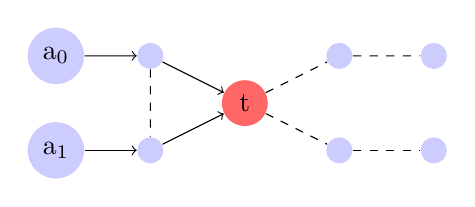
\begin{tikzpicture}
			  [scale=.6,auto=left,every node/.style={circle,fill=blue!20}]
			  \node (n1) at (1,3) {a$_0$};
			  \node (n2) at (3,3) { };
			  
	  		  \node (n3) at (1,1) {a$_1$};
			  \node (n4) at (3,1) { };
			  
			  \node[style={circle,fill=red!60}] (n5) at (5,2) {t};
			  
			  \node (n6) at (7,3) { };
			  \node (n7) at (7,1) { };
			  \node (n8) at (9,3) { };
			  \node (n9) at (9,1) { };
			  		  
			  \foreach \from/\to in {n1/n2,n2/n5,n3/n4,n4/n5}
			  \draw (\from) edge[->] (\to);
	
			  \foreach \from/\to in {n5/n6,n5/n7,n6/n8,n7/n9,n2/n4}
			  \draw (\from) edge[-,dashed] (\to);		  
			\end{tikzpicture}
			
			(a)\\
		\end{minipage}
		
		\bigskip
		\begin{minipage}[b]{0.9\linewidth}
			\centering
			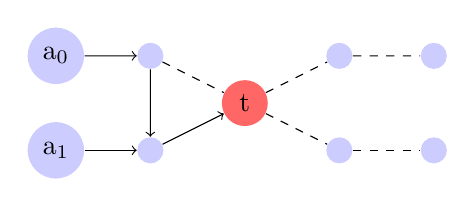
\begin{tikzpicture}
			  [scale=.6,auto=left,every node/.style={circle,fill=blue!20}]
			  \node (n1) at (1,3) {a$_0$};
			  \node (n2) at (3,3) { };
			  
	  		  \node (n3) at (1,1) {a$_1$};
			  \node (n4) at (3,1) { };
			  
			  \node[style={circle,fill=red!60}] (n5) at (5,2) {t};
			  
			  \node (n6) at (7,3) { };
			  \node (n7) at (7,1) { };
			  \node (n8) at (9,3) { };
			  \node (n9) at (9,1) { };
			  		  
			  \foreach \from/\to in {n1/n2,n3/n4,n4/n5,n2/n4}
			  \draw (\from) edge[->] (\to);
	
			  \foreach \from/\to in {n5/n6,n5/n7,n6/n8,n7/n9,n2/n5}
			  \draw (\from) edge[-,dashed] (\to);		  
			\end{tikzpicture}
			
			(b)\\
		\end{minipage}
	\end{center}
	\caption{\label{fig:prev_phi}
	     Ejemplos de emboscadas con dos agentes con valores de $\Phi$ de
	     $1.0$ para (a) dado que cubre dos caminos y $0.5$ para (b) dado que
	     cubre un camino. En el caso (b), se considera apenas un predecesor
	     del nodo $t$ de los dos predecesores posibles.
	}
\end{figure}

Sin embargo, esta m\'etrica penaliza casos donde no es posible alcanzar
una mejor emboscada, a\'un cuando se cuenta con suficientes agentes, debido
a la configuraci\'on del grafo y de las posiciones iniciales de estos. 
Ejemplos de estos casos pueden ser observados en la figura \ref{fig:error_phi}. En
la situaci\'on superior, se observa que a pesar de contar con cuatro agentes,
las dos salidas restantes no son alcanzables por estos sin pasar antes por el
nodo objetivo. Por otra parte, en la situaci\'on inferior, a pesar de que todas
las salidas son alcanzables por los agentes, no es posible alcanzar una
configuraci\'on de caminos capaz de cubrir todas las salidas. Para ambos
casos, a pesar de que la asignaci\'on de caminos es la mejor dadas las
condiciones iniciales, la m\'etrica originalmente planteada reporta resultados
sub\'optimos.

\begin{figure}[htb]
	\begin{center}
		\begin{minipage}[b]{0.9\linewidth}
			\centering
			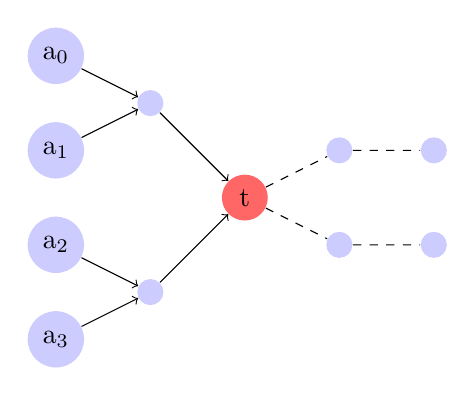
\begin{tikzpicture}
			  [scale=.6,auto=left,every node/.style={circle,fill=blue!20}]
			  \node (n11) at (1,7) {a$_0$};
			  \node (n12) at (1,5) {a$_1$};
			  \node (n2) at (3,6) { };
			  
	  		  \node (n31) at (1,3) {a$_2$};
	  		  \node (n32) at (1,1) {a$_3$};
			  \node (n4) at (3,2) { };
			  
			  \node[style={circle,fill=red!60}] (n5) at (5,4) {t};
			  
			  \node (n6) at (7,5) { };
			  \node (n7) at (7,3) { };
			  \node (n8) at (9,5) { };
			  \node (n9) at (9,3) { };
			  
			  \foreach \from/\to in {n11/n2,n12/n2,n2/n5,n31/n4,n32/n4,n4/n5}
			  \draw (\from) edge[->] (\to);
	
			  \foreach \from/\to in {n5/n6,n5/n7,n6/n8,n7/n9}
			  \draw (\from) edge[-,dashed] (\to);		  
			\end{tikzpicture}
			
			(a)\\
		\end{minipage}
		
		\bigskip
		\begin{minipage}[b]{0.9\linewidth}
			\centering
			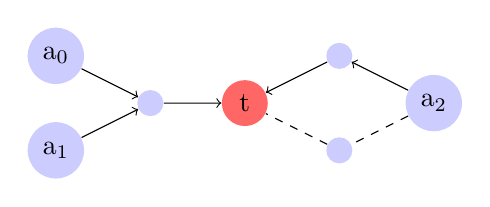
\begin{tikzpicture}
			  [scale=.6,auto=left,every node/.style={circle,fill=blue!20}]
			  \node (n11) at (1,3) {a$_0$};
			  \node (n12) at (1,1) {a$_1$};
			  \node (n2) at (3,2) { };
			  
	  		  \node (n3) at (9,2) {a$_2$};
			  \node (n41) at (7,3) { };
  			  \node (n42) at (7,1) { };
  			  
			  \node[style={circle,fill=red!60}] (n5) at (5,2) {t};
			  
			  \foreach \from/\to in {n11/n2,n12/n2,n2/n5,n3/n41,n41/n5}
			  \draw (\from) edge[->] (\to);
	
			  \foreach \from/\to in {n3/n42,n42/n5}
			  \draw (\from) edge[-,dashed] (\to);		  
			\end{tikzpicture}
			
			(b)
		\end{minipage}
	\end{center}
	\caption{\label{fig:error_phi}
	     Casos en los cuales la m\'etrica original pe\-na\-li\-za emboscadas
	     \'optimas. (a) Caso de no alcanzabilidad. (b) Caso de no existencia
	     de mejor asignaci\'on posible.}
\end{figure}

Por lo tanto, es necesario utilizar una nueva medida de emboscada
para poder discriminar correctamente entre las escapatorias que podr\'ian
ser cubiertas por alg\'un agente y aquellas que no. Esta nueva medida,
denotada por $\Phi^*$ (\ref{eq:new}) busca normalizar a los agentes utilizando
el tamaño de la m\'axima asociaci\'on de agentes a los nodos predecesores
del objetivo que \'estos son capaces de alcanzar. Se define $\Phi^*$ como:

\begin{small}
\begin{eqnarray}
 \Phi(t) &=& 
\dfrac{|\{ i : path(j) = <pos(j),\ \ldots,\ i,\ t>, j \in A\}|}
	  {|\{ y : (x,y) \in MaxMatching(BipG(G,A,t))\}|}
\label{eq:new}
\end{eqnarray}
\end{small}

\noindent
donde $BipG(G,A,t)$ define el grafo bipartito que asocia a agentes con
los nodos alcanzables por cada uno que sean predecesores del nodo objetivo
(\ref{eq:bipgraph}).
Este grafo se construye considerando como nodos el conjunto
de los agentes y el conjunto de los nodos predecesores alcanzables por alg\'un
agente (\ref{eq:bipgraphdst}). Por otra parte, los arcos provienen
de la matriz de alcanzabilidad entre agentes y predecesores (\ref{eq:bipgraphedges}).

\begin{small}
\begin{eqnarray}
BipG(G,A,t) & = & 
  (A\ \cup\ Dst(G,A,t),\ Edges(G,A,t)) \label{eq:bipgraph}\\
Dst(G,A,t) & = & Reachable(Reduced(G,t),\ A)\label{eq:bipgraphdst} \\
Edges(G,A,t) & = & \{ (x,y) : x \in A \wedge y \in Dst(G,A,t) \wedge\ \nonumber\\
& & \hspace{27pt} ScopeXY(G,A,t,x,y)\nonumber\\
& & \} \label{eq:bipgraphedges}\\
\nonumber\\
Reduced((V,E), t) & = & (V-\{t\}, E - \{<x,y>: x = t  \vee y = t\})\nonumber\\
Reachable(G,A) &=& \bigcup_{a \in A} Scope(G, pos(a))\nonumber\\
Scope((\{\},E), v) & = & \{\}\nonumber\\
Scope(G, v) & = & \{v\} \cup \bigcup_{w \in suc(G,v)}Scope(Reduced(G,v),w)\nonumber\\
\nonumber\\
ScopeXY(G,A,t,x,y) &=& x \in A \ \wedge\ y \in Scope(Reduced(G,t),pos(x))\nonumber
\end{eqnarray}
\end{small}

\noindent
y donde, asumiendo que el operador $argmax$ retorna el conjunto de mayor
tamaño que eval\'ue como cierta la condici\'on expuesta, se define
la m\'axima asociaci\'on de un grafo como (\ref{eq:mm})

\begin{small}
\begin{eqnarray}
MaxMatching((V,E)) & = & argmax_{m \subseteq E}( AtMostOnceSrc(m)\ \wedge\nonumber\\
				   &   & \hspace{43pt}AtMostOnceDst(m)\nonumber\\
				   &   & )
\label{eq:mm}
\end{eqnarray}
\end{small}

Una implementaci\'on real de esta m\'etrica debe usar un algoritmo de
c\'alculo de apareamiento en grafos bipartitos en tiempo polinomial\cite{Wes01}.
La definici\'on ac\'a planteada en t\'erminos de generaci\'on de subconjuntos
es utilizada \'unicamente por motivos de definici\'on formal. En cualquier caso,
el costo asociado a calcular la calidad de la emboscada no se ve reflejado en
el c\'alculo de las rutas para los agentes, dado que esto es un procedimiento
de validaci\'on experimental y no forma parte del algoritmo de \ambush ni de
sus va\-rian\-tes.

%\input{Astar}
\section{A*mbush}

In this section we propose \ambush, an $A^*$-based
algorithm that solves the ambush generation problem. 
It consists in a modification of $g$ function, that favours
path diversity. We will call this function $g'$.

Let $\Psi(v,i) = 1+(\# j : j \in A \wedge v \in path(j))$,
be the number of agents different from agent $i$, that have the 
node $v$ in their paths towards $t$ plus one. If an agent is not trying to 
reach node $t$ at the moment, or it has not performed the 
search for the node yet, it's path counts as empty. 
Therefore, the agent is not taken into account when calculating
$\Psi(v,i)$'s value. 

It is considered that $g'(pos(i),i) = 0$ for the initial node.
 Let $<v,w>$ be the next edge that should be expanded
from the node $v$, in any of the algorithm's iterations. In
these conditions, the expression that determines $g'$'s value
is $g'(w, i) = g'(v,i) + \lambda_i(<v,w>) \cdot \Psi(w,i)^2$.

Given that $\Psi(v,i) \geq 1$, the path determined by $A^*mbush$
is optimal under the new definition of $g'$. Hence, the properties of
 $A^*$ are preserved \cite{art2}. Nevertheless the path might not 
 be optimal for the original costs function $g$.

Note that $\Psi(v,i) = 1$ for every node $v$ that is not considered
in the path of any agent different to $i$. Similarly,
$\Psi(v,i) > 1$ in any other case. This condition allows the 
agents to consider exploring sub-optimal paths in the 
original graph. The less agents explore this routes, the greater
the chance given to other agents to travel trough them.

\subsection{Complexity}

It is possible to precompute the
function $\Psi$ for node cost's increment. If this function is stored
in a constant structure with fast access, the cost of calculating
$g'$ becomes equal to the cost of computing $g$.
Therefore, the only change if the algorithm's cost
 lays in the initial calculation of function $\Psi$.

The asymptotic complexity of $A^*mbush$ is:
$\bigO(|V|log(|V|) + |V|*h + |E| + |A|*|V| )$.

In the field of video games, the graphs of interest are
given by the polygonal division scheme of the map
\cite{book3,art1} (this polygons tend to have a small
amount of sides), according to the traversable regions 
and their respective adjacencies \cite{book3,art1}. 
Since the number of sides for the polygons is small, this 
graphs tend to have little density. In consequence,
$|E| \in \bigO(|V|)$, this means that the execution 
time of this methods for the graphs of interest in the
area of video games, is considered to be
$\bigO(|V|(log(|V|) + h + |A|) )$. 
The amortized cost of the increment function is $\bigO(|V|)$,
therefore, the amortized cost of the A$^*$mbush algorithm
equals the A$^*$ cost.

\begin{comment}
Figure
\ref{fig:graph_decomp} shows a clear example of a map 
broken into polygons. Each one of them is considered to
be a node in the search space. Two nodes are adjacent if 
their polygons share a common side. 

\begin{figure}[htp]
\centerline{\includegraphics[width=0.6\columnwidth]{figures/graph_decomposition.png}}
\caption{Up: Game map, the black blocks are the obstacles
              Down: Decomposition of the map into convex polygons}
\label{fig:graph_decomp}
\end{figure}
\end{comment}


\input{R-Ambush}
\input{SelfRAmbush}
\section{Experimentos}
\label{sec:experiments}

\begin{table}
	\caption{Calidad de emboscada para los grafos g1 y g2 utilizando distinto
	n\'umero de agentes (\#) ubicados en posiciones aleatorias distintas (arriba) y
	compartiendo la posici\'on inicial (abajo)}
	\label{tab:ambush_g}
	\centering
	\begin{small}
		\setlength{\tabcolsep}{4pt}
		\begin{tabular}{|c|cc|cc|cc|cc|}
			\hline
			\multicolumn{9}{|c|}{\textbf{g1 (60 pol\'igonos)}}\\
			\hline			
			\multirow{2}{*}{\textbf{\#}} &
			\multicolumn{2}{c|}{\textbf{\astar}} &
			\multicolumn{2}{c|}{\textbf{\ambush}} &
			\multicolumn{2}{c|}{\textbf{P}} &
			\multicolumn{2}{c|}{\textbf{SAR}}\\
			& $\Phi$ & $\Phi^*$ & $\Phi$ & $\Phi^*$&
			$\Phi$ & $\Phi^*$& $\Phi$ & $\Phi^*$\\
			\hline
			2  & 0.71 & 0.73 & 0.82 & 0.84 & 0.82 & 0.84 & 0.83 & 0.84\\
			5  & 0.89 & 0.90 & 0.99 & 1.00 & 0.99 & 1.00 & 0.99 & 1.00\\
			10 & 0.98 & 0.98 & 1.00 & 1.00 & 1.00 & 1.00 & 1.00 & 1.00\\
			20 & 0.97 & 0.99 & 0.98 & 1.00 & 0.98 & 1.00 & 0.98 & 1.00\\
			\hline
			\multicolumn{9}{|c|}{\textbf{g2 (85 pol\'igonos)}}\\
			\hline
			\multirow{2}{*}{\textbf{\#}} &
			\multicolumn{2}{c|}{\textbf{\astar}} &
			\multicolumn{2}{c|}{\textbf{\ambush}} &
			\multicolumn{2}{c|}{\textbf{P}} &
			\multicolumn{2}{c|}{\textbf{SAR}}\\
			& $\Phi$ & $\Phi^*$ & $\Phi$ & $\Phi^*$&
			$\Phi$ & $\Phi^*$& $\Phi$ & $\Phi^*$\\
			\hline
			2  & 0.65 & 0.67 & 0.87 & 0.89 & 0.87 & 0.89 & 0.88 & 0.90\\
			5  & 0.87 & 0.87 & 1.00 & 1.00 & 1.00 & 1.00 & 1.00 & 1.00\\
			10 & 0.95 & 0.95 & 1.00 & 1.00 & 1.00 & 1.00 & 1.00 & 1.00\\
			20 & 0.99 & 0.99 & 1.00 & 1.00 & 1.00 & 1.00 & 1.00 & 1.00\\
			\hline
		\end{tabular}
		
		\bigskip
		\begin{tabular}{|c|cc|cc|cc|cc|}
			\hline
			\multicolumn{9}{|c|}{\textbf{g1 (60 pol\'igonos)}}\\
			\hline			
			\multirow{2}{*}{\textbf{\#}} &
			\multicolumn{2}{c|}{\textbf{\astar}} &
			\multicolumn{2}{c|}{\textbf{\ambush}} &
			\multicolumn{2}{c|}{\textbf{P}} &
			\multicolumn{2}{c|}{\textbf{SAR}}\\
			& $\Phi$ & $\Phi^*$ & $\Phi$ & $\Phi^*$&
			$\Phi$ & $\Phi^*$& $\Phi$ & $\Phi^*$\\
			\hline
			2 & 0.50 & 0.50 & 0.81 & 0.81 & 0.81 & 0.81 & 0.83 & 0.83\\
			5 & 0.48 & 0.48 & 0.97 & 0.98 & 0.97 & 0.98 & 0.97 & 0.98\\
			10 & 0.46 & 0.46 & 0.96 & 0.96 & 0.96 & 0.96 & 0.94 & 0.95\\
			20 & 0.47 & 0.48 & 0.98 & 0.99 & 0.98 & 0.99 & 0.97 & 0.98\\
			\hline
			\multicolumn{9}{|c|}{\textbf{g2 (85 pol\'igonos)}}\\
			\hline
			\multirow{2}{*}{\textbf{\#}} &
			\multicolumn{2}{c|}{\textbf{\astar}} &
			\multicolumn{2}{c|}{\textbf{\ambush}} &
			\multicolumn{2}{c|}{\textbf{P}} &
			\multicolumn{2}{c|}{\textbf{SAR}}\\
			& $\Phi$ & $\Phi^*$ & $\Phi$ & $\Phi^*$&
			$\Phi$ & $\Phi^*$& $\Phi$ & $\Phi^*$\\
			\hline
			2 & 0.50 & 0.50 & 0.81 & 0.81 & 0.81 & 0.81 & 0.87 & 0.87\\
			5 & 0.46 & 0.46 & 0.94 & 0.94 & 0.94 & 0.94 & 0.96 & 0.96\\
			10 & 0.46 & 0.46 & 0.98 & 0.98 & 0.98 & 0.98 & 0.97 & 0.97\\
			20 & 0.47 & 0.47 & 0.98 & 0.98 & 0.98 & 0.98 & 0.98 & 0.98\\
			\hline
		\end{tabular}
	\end{small}
\end{table}

\begin{table}
	\caption{Calidad de emboscada para grafos tipo langosta
	con \textbf{n} nodos y n\'umero de agentes
	(\textbf{\#}) ubicados en posiciones aleatorias distintas (arriba) y
	compartiendo la posici\'on inicial (abajo)}
	\label{tab:ambush_lobster}
	\centering
	\begin{small}
		\setlength{\tabcolsep}{4pt}
		\begin{tabular}{|c|c|cc|cc|cc|cc|}
			\hline
			\multirow{2}{*}{\textbf{n}} &
			\multirow{2}{*}{\textbf{\#}} &
			\multicolumn{2}{c|}{\textbf{\astar}} &
			\multicolumn{2}{c|}{\textbf{\ambush}} &
			\multicolumn{2}{c|}{\textbf{P}} &
			\multicolumn{2}{c|}{\textbf{SAR}}\\
			& & $\Phi$ & $\Phi^*$ & $\Phi$ & $\Phi^*$&
			$\Phi$ & $\Phi^*$& $\Phi$ & $\Phi^*$\\
			\hline
			\multirow{4}{*}{$10^2$}
			 & 2 & 0.76 & 1.00 & 0.76 & 1.00 & 0.76 & 1.00 & 0.76 & 1.00\\
			 & 5 & 0.80 & 1.00 & 0.80 & 1.00 & 0.80 & 1.00 & 0.80 & 1.00\\
			 & 10 & 0.80 & 1.00 & 0.80 & 1.00 & 0.80 & 1.00 & 0.80 & 1.00\\
			 & 20 & 0.85 & 1.00 & 0.85 & 1.00 & 0.85 & 1.00 & 0.85 & 1.00\\
			\hline
			\multirow{4}{*}{$10^3$}
			 & 2 & 0.75 & 1.00 & 0.75 & 1.00 & 0.75 & 1.00 & 0.75 & 1.00\\
			 & 5 & 0.72 & 1.00 & 0.72 & 1.00 & 0.72 & 1.00 & 0.72 & 1.00\\
			 & 10 & 0.77 & 1.00 & 0.77 & 1.00 & 0.77 & 1.00 & 0.77 & 1.00\\
			 & 20 & 0.81 & 1.00 & 0.81 & 1.00 & 0.81 & 1.00 & 0.81 & 1.00\\
			 \hline
			\multirow{4}{*}{$10^4$}
			 & 2 & 0.71 & 1.00 & 0.71 & 1.00 & 0.71 & 1.00 & 0.71 & 1.00\\
			 & 5 & 0.69 & 1.00 & 0.69 & 1.00 & 0.69 & 1.00 & 0.69 & 1.00\\
			 & 10 & 0.77 & 1.00 & 0.77 & 1.00 & 0.77 & 1.00 & 0.77 & 1.00\\
			 & 20 & 0.78 & 1.00 & 0.78 & 1.00 & 0.78 & 1.00 & 0.78 & 1.00\\
			 \hline
		\end{tabular}
		
		\bigskip
		\begin{tabular}{|c|c|cc|cc|cc|cc|}
			\hline
			\multirow{2}{*}{\textbf{n}} &
			\multirow{2}{*}{\textbf{\#}} &
			\multicolumn{2}{c|}{\textbf{\astar}} &
			\multicolumn{2}{c|}{\textbf{\ambush}} &
			\multicolumn{2}{c|}{\textbf{P}} &
			\multicolumn{2}{c|}{\textbf{SAR}}\\
			& & $\Phi$ & $\Phi^*$ & $\Phi$ & $\Phi^*$&
			$\Phi$ & $\Phi^*$& $\Phi$ & $\Phi^*$\\
			\hline
			\multirow{4}{*}{$10^2$}
			 & 2 & 0.65 & 1.00 & 0.65 & 1.00 & 0.65 & 1.00 & 0.65 & 1.00\\
			 & 5 & 0.57 & 1.00 & 0.57 & 1.00 & 0.57 & 1.00 & 0.57 & 1.00\\
			 & 10 & 0.57 & 1.00 & 0.57 & 1.00 & 0.57 & 1.00 & 0.57 & 1.00\\
			 & 20 & 0.59 & 1.00 & 0.59 & 1.00 & 0.59 & 1.00 & 0.59 & 1.00\\
			\hline
			\multirow{4}{*}{$10^3$}
			 & 2 & 0.64 & 1.00 & 0.64 & 1.00 & 0.64 & 1.00 & 0.64 & 1.00\\
			 & 5 & 0.56 & 1.00 & 0.56 & 1.00 & 0.56 & 1.00 & 0.56 & 1.00\\
			 & 10 & 0.57 & 1.00 & 0.57 & 1.00 & 0.57 & 1.00 & 0.57 & 1.00\\
			 & 20 & 0.59 & 1.00 & 0.59 & 1.00 & 0.59 & 1.00 & 0.59 & 1.00\\
			 \hline
			\multirow{4}{*}{$10^4$}
			 & 2 & 0.70 & 1.00 & 0.70 & 1.00 & 0.70 & 1.00 & 0.70 & 1.00\\
			 & 5 & 0.61 & 1.00 & 0.61 & 1.00 & 0.61 & 1.00 & 0.61 & 1.00\\
			 & 10 & 0.56 & 1.00 & 0.56 & 1.00 & 0.56 & 1.00 & 0.56 & 1.00\\
			 & 20 & 0.58 & 1.00 & 0.58 & 1.00 & 0.58 & 1.00 & 0.58 & 1.00\\
			 \hline
		\end{tabular}
	\end{small}
\end{table}


Para cada experimento se estudian cuatro algoritmos:
una implementaci\'on base de \astar\ que sirve de referencia,
\ambush, \pambush\ (\textbf{P}) con mecanismo de prioridad determinado por
la distancia real de los agentes a la meta y, finalmente, \sarambush\
(\textbf{SAR}).

\begin{comment}
\begin{figure}[htb]
	\begin{center}
		\includegraphics[scale=0.23]{figures/g1.png}
		\includegraphics[scale=0.23]{figures/g2.png}
	\end{center}
	\caption{\label{fig:gs}
	     \textbf{Arriba:} Mapa 1 poligonalizado (60 pol\'igonos).
	     \textbf{Abajo:} Mapa 2 poligonalizado (85 pol\'igonos).
     }
\end{figure}
\end{comment}

Se utilizaron diversas topolog\'ias de grafos, para las cuales
se generan grafos aleatoriamente de distintos tamaños. Para cada
experimento se efect\'uan 100 disposiciones distintas de agentes
y del nodo objetivo. En los casos donde se referencia
que todos los agentes parten de la misma posici\'on inicial, \'esta es
com\'un para todos ellos, sin embargo, su disposici\'on es aleatoria.
Para cada uno de estos algoritmos se muestra el valor de emboscada
utilizando la m\'etrica originalmente propuesta y utilizando la
m\'etrica propuesta en el presente trabajo. Se prob\'o variar el
n\'umero de agentes con el fin de mostrar su impacto en el grado de emboscada.
Adem\'as, se muestran resultados con las dos instancias de mapas ($g1$ y $g2$)
presentadas en el trabajo previo \cite{FGC12} con 60 y 85 nodos
respectivamente. Estos mapas provienen de la poligonalizaci\'on de mapas
de juego en pol\'igonos. Este tipo de grafos son ampliamente utilizados
en juegos\cite{MF09}.

Para los experimentos con los grafos iniciales (g1 y g2), se mostr\'o
la efectividad de las tres variantes propuestas con respecto a \astar.
Adicionalmente, se evidencia en este y otros experimentos la mejora
al evaluar el grado de emboscada utilizando la m\'etrica nueva, dado
que la original subeval\'ua va\-rios casos de emboscada.
Los resultados de este experimento se pueden evidenciar en la tabla
\ref{tab:ambush_g}. Asimismo, en este y en los experimentos subsiguientes,
se puede apreciar como en los casos donde los agentes parten de una misma
posici\'on inicial, las diversas variantes de \ambush\ logran efectivamente
mejorar el grado de emboscada, incluso con un n\'umero bajo de agentes
involucrados.

\begin{table}
	\caption{Calidad de emboscada para grafos tipo Erd\H{o}s-R{\'e}nyi
	con \textbf{n} nodos, probabilidad de conexi\'on 0.7 y n\'umero de agentes
	(\textbf{\#}) ubicados en posiciones aleatorias distintas (arriba) y
	compartiendo la posici\'on inicial (abajo)}
	\label{tab:ambush_er}
	\centering
	\begin{small}
		\setlength{\tabcolsep}{4pt}
		\begin{tabular}{|c|c|cc|cc|cc|cc|}
			\hline
			\multirow{2}{*}{\textbf{n}} &
			\multirow{2}{*}{\textbf{\#}} &
			\multicolumn{2}{c|}{\textbf{\astar}} &
			\multicolumn{2}{c|}{\textbf{\ambush}} &
			\multicolumn{2}{c|}{\textbf{P}} &
			\multicolumn{2}{c|}{\textbf{SAR}}\\
			& & $\Phi$ & $\Phi^*$ & $\Phi$ & $\Phi^*$&
			$\Phi$ & $\Phi^*$& $\Phi$ & $\Phi^*$\\
			\hline
			\multirow{4}{*}{$10^2$}
			 & 2 & 0.39 & 0.98 & 0.41 & 1.00 & 0.41 & 1.00 & 0.41 & 1.00\\
			 & 5 & 0.32 & 0.93 & 0.35 & 0.98 & 0.35 & 0.98 & 0.35 & 0.98\\
			 & 10 & 0.34 & 0.88 & 0.38 & 0.95 & 0.38 & 0.95 & 0.38 & 0.95\\
			 & 20 & 0.49 & 0.89 & 0.53 & 0.94 & 0.53 & 0.94 & 0.53 & 0.94\\
			\hline
			\multirow{4}{*}{$10^3$}
			 & 2 & 0.50 & 1.00 & 0.50 & 1.00 & 0.50 & 1.00 & 0.50 & 1.00\\
			 & 5 & 0.43 & 0.96 & 0.45 & 0.99 & 0.45 & 0.99 & 0.45 & 0.99\\
			 & 10 & 0.42 & 0.92 & 0.47 & 0.99 & 0.47 & 0.99 & 0.47 & 0.99\\
			 & 20 & 0.40 & 0.82 & 0.47 & 0.94 & 0.47 & 0.94 & 0.47 & 0.94\\
			 \hline
			\multirow{4}{*}{$10^4$}
			 & 2 & 0.47 & 0.99 & 0.48 & 1.00 & 0.48 & 1.00 & 0.48 & 1.00\\
			 & 5 & 0.44 & 0.99 & 0.45 & 1.00 & 0.45 & 1.00 & 0.45 & 1.00\\
			 & 10 & 0.44 & 0.95 & 0.47 & 1.00 & 0.47 & 1.00 & 0.47 & 1.00\\
			 & 20 & 0.44 & 0.87 & 0.50 & 0.98 & 0.50 & 0.98 & 0.50 & 0.98\\
			 \hline
		\end{tabular}
		
		\bigskip
		\begin{tabular}{|c|c|cc|cc|cc|cc|}
			\hline
			\multirow{2}{*}{\textbf{n}} &
			\multirow{2}{*}{\textbf{\#}} &
			\multicolumn{2}{c|}{\textbf{\astar}} &
			\multicolumn{2}{c|}{\textbf{\ambush}} &
			\multicolumn{2}{c|}{\textbf{P}} &
			\multicolumn{2}{c|}{\textbf{SAR}}\\
			& & $\Phi$ & $\Phi^*$ & $\Phi$ & $\Phi^*$&
			$\Phi$ & $\Phi^*$& $\Phi$ & $\Phi^*$\\
			\hline
			\multirow{4}{*}{$10^2$}
			 & 2 & 0.43 & 0.68 & 0.69 & 0.94 & 0.69 & 0.94 & 0.69 & 0.94\\
			 & 5 & 0.27 & 0.52 & 0.59 & 0.92 & 0.59 & 0.92 & 0.60 & 0.92\\
			 & 10 & 0.25 & 0.52 & 0.54 & 0.96 & 0.54 & 0.96 & 0.54 & 0.96\\
			 & 20 & 0.20 & 0.49 & 0.48 & 0.93 & 0.48 & 0.93 & 0.47 & 0.92\\
			\hline
			\multirow{4}{*}{$10^3$}
			 & 2 & 0.40 & 0.63 & 0.74 & 0.97 & 0.74 & 0.97 & 0.74 & 0.97\\
			 & 5 & 0.15 & 0.52 & 0.56 & 0.93 & 0.56 & 0.93 & 0.56 & 0.93\\
			 & 10 & 0.09 & 0.47 & 0.49 & 0.93 & 0.49 & 0.93 & 0.48 & 0.91\\
			 & 20 & 0.06 & 0.46 & 0.42 & 0.93 & 0.42 & 0.93 & 0.39 & 0.89\\
			 \hline
			\multirow{4}{*}{$10^4$}
			 & 2 & 0.22 & 0.81 & 0.38 & 0.97 & 0.38 & 0.97 & 0.38 & 0.97\\
			 & 5 & 0.10 & 0.64 & 0.39 & 0.92 & 0.39 & 0.92 & 0.39 & 0.92\\
			 & 10 & 0.05 & 0.65 & 0.32 & 0.94 & 0.32 & 0.94 & 0.32 & 0.94\\
			 & 20 & 0.02 & 0.69 & 0.22 & 0.96 & 0.22 & 0.96 & 0.20 & 0.94\\
			 \hline
		\end{tabular}
	\end{small}
\end{table}


Para demostrar la necesidad de la creaci\'on de esta nueva m\'etrica,
se procedi\'o a probar la efectividad del algoritmo utilizando grafos
con poca diversidad posible de caminos, en los cuales, no es posible
generar emboscadas totales en muchos casos. Para esto, se utilizaron
grafos tipo langosta (Lobster graphs) \cite{Gal09} y grafos generados
bajo el modelo propuesto por Erd\H{o}s y R{\'e}nyi (grafos binomiales)
\cite{ER59}, siendo \'estos convertidos a grafos dirigidos con el fin de
reducir el n\'umero de componentes fuertemente conexas. Los experimentos sobre
grafos tipo langosta representan el peor caso para la m\'etrica originalmente
propuesta; dado que estos son \'arboles, existe s\'olo un camino entre
cualquier par de nodos, por lo que no es posible cubrir aquellos nodos
es\-ca\-pa\-to\-ria sin pasar por el nodo objetivo. En la tabla
\ref{tab:ambush_lobster} se muestran los resultados obtenidos utilizando
este tipo de grafos.
An\'alogamente, en la tabla \ref{tab:ambush_er} se muestran los resultados
para el modelo Erd{\H{o}s-R{\'e}nyi. Para este tipo de grafos, dada la
e\-xis\-ten\-cia de m\'ultiples caminos entre un par de nodos, no s\'olo se
evidencia una mejora de la nueva m\'etrica con respecto a la anterior, sino
tambi\'en de las variantes de \ambush\ con respecto a \astar. La mejora
aportada por \ambush\ parece casi imperceptible al ser estudiada
con la m\'etrica original, sin embargo, al ser analizado con la nueva
m\'etrica, se hace notar que el grado de emboscada alcanzado tiende a ser
el m\'aximo posible.

\begin{table}
	\caption{Calidad de emboscada para grafos tipo grilla cuadrada
	utilizando distinto tamaño de grilla (\textbf{n x n}) y n\'umero de agentes
	(\textbf{\#}) ubicados en posiciones aleatorias distintas (arriba) y
	compartiendo la posici\'on inicial (abajo)}
	\label{tab:ambush_grid}
	\centering
	\begin{small}
		\setlength{\tabcolsep}{4pt}
		\begin{tabular}{|c|c|cc|cc|cc|cc|}
			\hline
			\multirow{2}{*}{\textbf{n}} &
			\multirow{2}{*}{\textbf{\#}} &
			\multicolumn{2}{c|}{\textbf{\astar}} &
			\multicolumn{2}{c|}{\textbf{\ambush}} &
			\multicolumn{2}{c|}{\textbf{P}} &
			\multicolumn{2}{c|}{\textbf{SAR}}\\
			& & $\Phi$ & $\Phi^*$ & $\Phi$ & $\Phi^*$&
			$\Phi$ & $\Phi^*$& $\Phi$ & $\Phi^*$\\
			\hline
			\multirow{4}{*}{10}
			 & 2 & 0.88 & 0.89 & 0.98 & 0.98 & 0.98 & 0.98 & 0.98 & 0.98\\
			 & 5 & 0.65 & 0.65 & 0.95 & 0.95 & 0.95 & 0.95 & 0.95 & 0.95\\
			 & 10 & 0.72 & 0.72 & 0.92 & 0.92 & 0.92 & 0.92 & 0.93 & 0.93\\
			 & 20 & 0.83 & 0.83 & 0.96 & 0.96 & 0.96 & 0.96 & 0.96 & 0.96\\
			\hline
			\multirow{4}{*}{20}
			 & 2 & 0.89 & 0.90 & 1.00 & 1.00 & 1.00 & 1.00 & 1.00 & 1.00\\
			 & 5 & 0.65 & 0.65 & 0.98 & 0.98 & 0.98 & 0.98 & 0.97 & 0.98\\
			 & 10 & 0.66 & 0.66 & 0.96 & 0.96 & 0.96 & 0.96 & 0.96 & 0.96\\
			 & 20 & 0.78 & 0.78 & 0.97 & 0.97 & 0.97 & 0.97 & 0.97 & 0.97\\
			 \hline
			\multirow{4}{*}{100}
			 & 2 & 0.89 & 0.89 & 1.00 & 1.00 & 1.00 & 1.00 & 1.00 & 1.00\\
			 & 5 & 0.68 & 0.68 & 1.00 & 1.00 & 1.00 & 1.00 & 1.00 & 1.00\\
			 & 10 & 0.58 & 0.58 & 0.99 & 0.99 & 0.99 & 0.99 & 0.99 & 0.99\\
			 & 20 & 0.74 & 0.74 & 0.99 & 0.99 & 0.99 & 0.99 & 0.99 & 0.99\\
			 \hline
		\end{tabular}
		
		\bigskip
		\begin{tabular}{|c|c|cc|cc|cc|cc|}
			\hline
			\multirow{2}{*}{\textbf{n}} &
			\multirow{2}{*}{\textbf{\#}} &
			\multicolumn{2}{c|}{\textbf{\astar}} &
			\multicolumn{2}{c|}{\textbf{\ambush}} &
			\multicolumn{2}{c|}{\textbf{P}} &
			\multicolumn{2}{c|}{\textbf{SAR}}\\
			& & $\Phi$ & $\Phi^*$ & $\Phi$ & $\Phi^*$&
			$\Phi$ & $\Phi^*$& $\Phi$ & $\Phi^*$\\
			\hline
			\multirow{4}{*}{10}
			 & 2 & 0.50 & 0.49 & 0.98 & 0.98 & 0.98 & 0.98 & 0.98 & 0.98\\
			 & 5 & 0.20 & 0.20 & 0.89 & 0.89 & 0.89 & 0.89 & 0.89 & 0.89\\
			 & 10 & 0.16 & 0.16 & 0.89 & 0.89 & 0.89 & 0.89 & 0.83 & 0.83\\
			 & 20 & 0.16 & 0.16 & 0.91 & 0.91 & 0.91 & 0.91 & 0.82 & 0.82\\
			\hline
			\multirow{4}{*}{20}
			 & 2 & 0.50 & 0.49 & 0.99 & 0.99 & 0.99 & 0.99 & 0.99 & 0.99\\
			 & 5 & 0.20 & 0.20 & 0.96 & 0.96 & 0.96 & 0.96 & 0.97 & 0.97\\
			 & 10 & 0.14 & 0.14 & 0.97 & 0.97 & 0.97 & 0.97 & 0.93 & 0.93\\
			 & 20 & 0.14 & 0.14 & 0.96 & 0.96 & 0.96 & 0.96 & 0.93 & 0.93\\
			 \hline
			\multirow{4}{*}{100}
			 & 2 & 0.50 & 0.50 & 1.00 & 1.00 & 1.00 & 1.00 & 1.00 & 1.00\\
			 & 5 & 0.20 & 0.20 & 1.00 & 1.00 & 1.00 & 1.00 & 1.00 & 1.00\\
		  	 & 10 & 0.13 & 0.13 & 0.99 & 0.99 & 0.99 & 0.99 & 0.98 & 0.98\\
			 & 20 & 0.13 & 0.13 & 1.00 & 0.99 & 1.00 & 0.99 & 0.98 & 0.98\\
			 \hline
		\end{tabular}
	\end{small}
\end{table}


\begin{table}
	\caption{Calidad de emboscada para grafos tipo Watts-Strotgatz small-world
	utilizando distinto n\'umero de nodos, 10 vecinos cercanos, probabilidad
	de reconexi\'on 0.5 y n\'umero de agentes
	(\textbf{\#}) ubicados en posiciones aleatorias distintas (arriba) y
	compartiendo la posici\'on inicial (abajo)}
	\label{tab:ambush_watts}
	\centering
	\begin{small}
		\setlength{\tabcolsep}{4pt}
		\begin{tabular}{|c|c|cc|cc|cc|cc|}
			\hline
			\multirow{2}{*}{\textbf{n}} &
			\multirow{2}{*}{\textbf{\#}} &
			\multicolumn{2}{c|}{\textbf{\astar}} &
			\multicolumn{2}{c|}{\textbf{\ambush}} &
			\multicolumn{2}{c|}{\textbf{P}} &
			\multicolumn{2}{c|}{\textbf{SAR}}\\
			& & $\Phi$ & $\Phi^*$ & $\Phi$ & $\Phi^*$&
			$\Phi$ & $\Phi^*$& $\Phi$ & $\Phi^*$\\
			\hline
			\multirow{4}{*}{$10^2$}
			 & 2 & 0.94 & 0.94 & 1.00 & 0.99 & 1.00 & 0.99 & 1.00 & 0.99\\
			 & 5 & 0.77 & 0.78 & 0.96 & 0.98 & 0.96 & 0.98 & 0.96 & 0.98\\
			 & 10 & 0.68 & 0.68 & 0.97 & 0.97 & 0.97 & 0.97 & 0.97 & 0.97\\
			 & 20 & 0.84 & 0.84 & 1.00 & 1.00 & 1.00 & 1.00 & 1.00 & 1.00\\
			\hline
			\multirow{4}{*}{$10^3$}
			 & 2 & 0.95 & 0.95 & 1.00 & 1.00 & 1.00 & 1.00 & 1.00 & 1.00\\
			 & 5 & 0.79 & 0.79 & 1.00 & 1.00 & 1.00 & 1.00 & 1.00 & 1.00\\
			 & 10 & 0.66 & 0.67 & 1.00 & 1.00 & 1.00 & 1.00 & 1.00 & 1.00\\
			 & 20 & 0.86 & 0.86 & 1.00 & 1.00 & 1.00 & 1.00 & 1.00 & 1.00\\
			 \hline
			\multirow{4}{*}{$10^4$}
			 & 2 & 0.95 & 0.95 & 1.00 & 1.00 & 1.00 & 1.00 & 1.00 & 1.00\\
			 & 5 & 0.82 & 0.82 & 1.00 & 1.00 & 1.00 & 1.00 & 1.00 & 1.00\\
			 & 10 & 0.68 & 0.68 & 1.00 & 1.00 & 1.00 & 1.00 & 1.00 & 1.00\\
			 & 20 & 0.87 & 0.87 & 1.00 & 1.00 & 1.00 & 1.00 & 1.00 & 1.00\\
			 \hline
		\end{tabular}
		
		\bigskip
		\begin{tabular}{|c|c|cc|cc|cc|cc|}
			\hline
			\multirow{2}{*}{\textbf{n}} &
			\multirow{2}{*}{\textbf{\#}} &
			\multicolumn{2}{c|}{\textbf{\astar}} &
			\multicolumn{2}{c|}{\textbf{\ambush}} &
			\multicolumn{2}{c|}{\textbf{P}} &
			\multicolumn{2}{c|}{\textbf{SAR}}\\
			& & $\Phi$ & $\Phi^*$ & $\Phi$ & $\Phi^*$&
			$\Phi$ & $\Phi^*$& $\Phi$ & $\Phi^*$\\
			\hline
			\multirow{4}{*}{$10^2$}
			 & 2 & 0.50 & 0.49 & 0.93 & 0.93 & 0.93 & 0.93 & 0.93 & 0.93\\
			 & 5 & 0.20 & 0.20 & 0.89 & 0.89 & 0.89 & 0.89 & 0.89 & 0.89\\
			 & 10 & 0.11 & 0.11 & 0.89 & 0.89 & 0.89 & 0.89 & 0.88 & 0.88\\
			 & 20 & 0.10 & 0.10 & 0.80 & 0.80 & 0.80 & 0.80 & 0.78 & 0.78\\
			\hline
			\multirow{4}{*}{$10^3$}
			 & 2 & 0.50 & 0.49 & 0.99 & 0.98 & 0.99 & 0.98 & 0.99 & 0.98\\
			 & 5 & 0.20 & 0.20 & 0.99 & 0.99 & 0.99 & 0.99 & 0.99 & 0.99\\
			 & 10 & 0.11 & 0.11 & 0.99 & 0.99 & 0.99 & 0.99 & 0.99 & 0.99\\
			 & 20 & 0.10 & 0.10 & 1.00 & 1.00 & 1.00 & 1.00 & 1.00 & 1.00\\
			 \hline
			\multirow{4}{*}{$10^4$}
			 & 2 & 0.50 & 0.50 & 1.00 & 0.99 & 1.00 & 0.99 & 1.00 & 0.99\\
			 & 5 & 0.20 & 0.20 & 1.00 & 1.00 & 1.00 & 1.00 & 1.00 & 1.00\\
			 & 10 & 0.11 & 0.11 & 0.99 & 0.99 & 0.99 & 0.99 & 1.00 & 1.00\\
			 & 20 & 0.11 & 0.11 & 1.00 & 1.00 & 1.00 & 1.00 & 1.00 & 1.00\\
			 \hline
		\end{tabular}
	\end{small}
\end{table}


\begin{table}
	\caption{Calidad de emboscada para grafos tipo Navigable Small-World 
	utilizando conecciones de corto alcance de tamaño unitario y cinco conexiones
	de largo alcance por nodo, n\'umero de agentes (\textbf{\#}) ubicados en
	posiciones aleatorias distintas (arriba) y compartiendo la posici\'on
	inicial (abajo)}
	\label{tab:ambush_nswg}
	\centering
	\begin{small}
		\setlength{\tabcolsep}{4pt}
		\begin{tabular}{|c|c|cc|cc|cc|cc|}
			\hline
			\multirow{2}{*}{\textbf{n}} &
			\multirow{2}{*}{\textbf{\#}} &
			\multicolumn{2}{c|}{\textbf{\astar}} &
			\multicolumn{2}{c|}{\textbf{\ambush}} &
			\multicolumn{2}{c|}{\textbf{P}} &
			\multicolumn{2}{c|}{\textbf{SAR}}\\
			& & $\Phi$ & $\Phi^*$ & $\Phi$ & $\Phi^*$&
			$\Phi$ & $\Phi^*$& $\Phi$ & $\Phi^*$\\
			\hline
			\multirow{4}{*}{$10$}
			 & 2 & 0.93 & 0.94 & 0.99 & 1.00 & 0.99 & 1.00 & 0.99 & 1.00\\
			 & 5 & 0.79 & 0.79 & 0.96 & 0.97 & 0.96 & 0.97 & 0.97 & 0.97\\
			 & 10 & 0.66 & 0.68 & 0.93 & 0.96 & 0.93 & 0.96 & 0.93 & 0.96\\
			 & 20 & 0.77 & 0.81 & 0.96 & 1.00 & 0.96 & 1.00 & 0.96 & 1.00\\
			\hline
			\multirow{4}{*}{$20$}
			 & 2 & 0.93 & 0.94 & 0.99 & 1.00 & 0.99 & 1.00 & 0.99 & 1.00\\
			 & 5 & 0.85 & 0.85 & 1.00 & 1.00 & 1.00 & 1.00 & 1.00 & 1.00\\
			 & 10 & 0.71 & 0.72 & 0.99 & 0.99 & 0.99 & 0.99 & 0.99 & 0.99\\
			 & 20 & 0.77 & 0.78 & 0.99 & 1.00 & 0.99 & 1.00 & 0.99 & 1.00\\
			 \hline
			\multirow{4}{*}{$50$}
			 & 2 & 0.95 & 0.95 & 1.00 & 1.00 & 1.00 & 1.00 & 1.00 & 1.00\\
			 & 5 & 0.85 & 0.85 & 1.00 & 1.00 & 1.00 & 1.00 & 1.00 & 1.00\\
			 & 10 & 0.73 & 0.73 & 1.00 & 1.00 & 1.00 & 1.00 & 1.00 & 1.00\\
			 & 20 & 0.77 & 0.78 & 0.99 & 1.00 & 0.99 & 1.00 & 0.99 & 1.00\\
			 \hline
			\multirow{4}{*}{$100$}
			 & 2 & 0.98 & 0.98 & 1.00 & 1.00 & 1.00 & 1.00 & 1.00 & 1.00\\
			 & 5 & 0.84 & 0.84 & 1.00 & 1.00 & 1.00 & 1.00 & 1.00 & 1.00\\
			 & 10 & 0.72 & 0.72 & 1.00 & 1.00 & 1.00 & 1.00 & 1.00 & 1.00\\
			 & 20 & 0.77 & 0.77 & 1.00 & 1.00 & 1.00 & 1.00 & 1.00 & 1.00\\
			 \hline
		\end{tabular}
		
		\bigskip
		\begin{tabular}{|c|c|cc|cc|cc|cc|}
			\hline
			\multirow{2}{*}{\textbf{n}} &
			\multirow{2}{*}{\textbf{\#}} &
			\multicolumn{2}{c|}{\textbf{\astar}} &
			\multicolumn{2}{c|}{\textbf{\ambush}} &
			\multicolumn{2}{c|}{\textbf{P}} &
			\multicolumn{2}{c|}{\textbf{SAR}}\\
			& & $\Phi$ & $\Phi^*$ & $\Phi$ & $\Phi^*$&
			$\Phi$ & $\Phi^*$& $\Phi$ & $\Phi^*$\\
			\hline
			\multirow{4}{*}{$10$}
			& 2 & 0.50 & 0.50 & 0.94 & 0.94 & 0.94 & 0.94 & 0.94 & 0.94\\
			& 5 & 0.20 & 0.21 & 0.95 & 0.96 & 0.95 & 0.96 & 0.95 & 0.96\\
			& 10 & 0.10 & 0.11 & 0.85 & 0.86 & 0.85 & 0.86 & 0.85 & 0.86\\
			& 20 & 0.09 & 0.10 & 0.92 & 0.96 & 0.92 & 0.96 & 0.84 & 0.88\\
			\hline
			\multirow{4}{*}{$20$}
			& 2 & 0.50 & 0.50 & 0.99 & 0.99 & 0.99 & 0.99 & 0.99 & 0.99\\
			& 5 & 0.20 & 0.20 & 0.98 & 0.98 & 0.98 & 0.98 & 0.98 & 0.98\\
			& 10 & 0.10 & 0.10 & 0.93 & 0.94 & 0.93 & 0.94 & 0.93 & 0.94\\
			& 20 & 0.08 & 0.08 & 0.98 & 0.99 & 0.98 & 0.99 & 0.97 & 0.99\\
			\hline
			\multirow{4}{*}{$50$}
			& 2 & 0.50 & 0.50 & 1.00 & 1.00 & 1.00 & 1.00 & 1.00 & 1.00\\
			& 5 & 0.20 & 0.20 & 0.99 & 0.99 & 0.99 & 0.99 & 0.99 & 0.99\\
			& 10 & 0.10 & 0.10 & 0.99 & 0.99 & 0.99 & 0.99 & 0.99 & 0.99\\
			& 20 & 0.08 & 0.08 & 1.00 & 1.00 & 1.00 & 1.00 & 1.00 & 1.00\\
			 \hline
			\multirow{4}{*}{$100$}
			& 2 & 0.50 & 0.50 & 1.00 & 1.00 & 1.00 & 1.00 & 1.00 & 1.00\\
			& 5 & 0.20 & 0.20 & 1.00 & 1.00 & 1.00 & 1.00 & 1.00 & 1.00\\
			& 10 & 0.10 & 0.10 & 1.00 & 1.00 & 1.00 & 1.00 & 1.00 & 1.00\\
			& 20 & 0.07 & 0.07 & 0.99 & 0.99 & 0.99 & 0.99 & 0.98 & 0.98\\
			\hline
		\end{tabular}
	\end{small}
\end{table}


Los dem\'as grafos utilizados son de varios tipos provenientes de la
literatura. El primer tipo de grafos generados explorado son los grafos
en grilla cuadrada con 8-conectividad, los cuales son muy comunes en el
desarrollo de juegos debido a la eficacia en la determinaci\'on de caminos
y en la ubicaci\'on del agente en una de las ca\-si\-llas \cite{MF09}.
Los resultados de este experimento se pueden apreciar en la tabla
\ref{tab:ambush_grid}. A medida que el grafo se hace m\'as grande, la
calidad media de emboscada se hace mayor, sin embargo, a\'un en grafos
pequeños se muestra que la emboscada se alcanza efectivamente. Para este
tipo de grafos ambas m\'etricas reportan los mismos valores dado que la
grilla se encuentra completamente conectada, siendo posible alcanzar a
cualquier nodo por m\'as de una v\'ia. De esta forma,
ambos conjuntos, el de predecesores y el de asociaci\'on de agentes a
nodos son el mismo, por lo que el factor de normalizaci\'on act\'ua de la
misma forma en ambas m\'etricas. Este fen\'omeno no se aprecia en los otros
tipos de grafos estudiados.

Seguidamente se experiment\'o con grafos con propiedad de mundo-pequeño
(Small-World Networks) \cite{WS98}. En este tipo de grafos
la mayor\'ia de los nodos no son vecinos de los dem\'as, sin embargo,
la mayor\'ia son alcanzables por cualquier otro utilizando caminos con
un n\'umero corto de pasos. Este tipo de grafos podr\'ian ser dif\'iciles
para un m\'etodo como \ambush\ debido a esta propiedad, al no ofrecer suficiente
distancia para que los agentes se alejen imposibilitando as\'i alcanzar la
emboscada. Sin embargo, en las tablas \ref{tab:ambush_watts} y \ref{tab:ambush_nswg}
se muestra que el algoritmo es capaz de so\-bre\-lle\-var esta situaci\'on y lograr
emboscadas perfectas en muchos de los casos. Los tipos de grafos con esta
propiedad es\-tu\-dia\-dos son los propuestos por Watts y Strogatz \cite{WS98}
y el propuesto por Kleinberg \cite{Kle00}.

Finalmente, se realizaron experimentos con el modelo de grafos propuesto
por Dorogovtsev y Mendes \cite{DM02}. El cual produce grafos planares,
similares a los utilizados en el \'area de inter\'es. Bajo este tipo
de grafos, si bien el grado de emboscada alcanzado fue menor con respecto
a los otros tipos utilizados, se mostr\'o un incremento significativo
de este con respecto al algoritmo base probado \astar.

\end{document}
\section{Cosas del formato que es mejor no borrar aun}

Displayed equations or formulas are centered and set on a separate
line (with an extra line or halfline space above and below). Displayed
expressions should be numbered for reference. The numbers should be
consecutive within each section or within the contribution,
with numbers enclosed in parentheses and set on the right margin --
which is the default if you use the \emph{equation} environment, e.g.,
\begin{equation}
  \psi (u) = \int_{o}^{T} \left[\frac{1}{2}
  \left(\Lambda_{o}^{-1} u,u\right) + N^{\ast} (-u)\right] dt \;  .
\end{equation}

Equations should be punctuated in the same way as ordinary
text but with a small space before the end punctuation mark.


\begin{figure}
\centering
%\includegraphics[height=6.2cm]{eijkel2}
\caption{One kernel at $x_s$ (\emph{dotted kernel}) or two kernels at
$x_i$ and $x_j$ (\textit{left and right}) lead to the same summed estimate
at $x_s$. This shows a figure consisting of different types of
lines. Elements of the figure described in the caption should be set in
italics, in parentheses, as shown in this sample caption.}
\label{fig:example}
\end{figure}

\subsection{Program Code}

Program listings or program commands in the text are normally set in
typewriter font, e.g., CMTT10 or Courier.

\medskip

\noindent
{\it Example of a Computer Program}
\begin{verbatim}
blabla el codigo
\end{verbatim}
%
\noindent
{\small (Example from Jensen K., Wirth N. (1991) Pascal user manual and
report. Springer, New York)}

\subsection{Citations}

For citations in the text please use
square brackets and consecutive numbers: \cite{jour}, \cite{lncschap},
\cite{proceeding1} -- provided automatically
by \LaTeX 's \verb|\cite| \dots\verb|\bibitem| mechanism.

\begin{thebibliography}{4}

\bibitem{book1}
T.~Cormen, C.~Leiserson, R.~Rivest and C. Stein, \emph{Introduction to Algorithms, 3rd ed}.\hskip 1em plus 0.5em minus 0.4em\relax
  The MIT Press, 2009.
  
\bibitem{book2}
M.~Gendreau and J.~Potvin, \emph{Handbook of Metaheuristics, 2nd ed}.\hskip 1em plus 0.5em minus 0.4em\relax
  Springer, 2010.  

\bibitem{book3}
I.~Millington and J.~Funge, \emph{Artificial Intelligence for Games, 2nd ed}.\hskip 1em plus 0.5em minus 0.4em\relax
  Morgan Kaufmann Publishers, 2009.  

\bibitem{book4}
S.~Russell and P.~Norvig, \emph{Artificial Intelligence: A Modern Approach, 2nd ed}.\hskip 1em plus 0.5em minus 0.4em\relax
  	Prentice-Hall, Englewood Cliffs, NJ,, 1993.  
  
\bibitem{art1}
X.~Cui and H.~Shii, ``Direction oriented pathfinding in video games,'' \emph{International Journal of Artificial Intelligence  \& applications 2}, 2011.

\bibitem{art2}
P.~Hart, N.~Nilsson and B.~Raphael, ``Correction to “a formal basis for the heuristic determination of minimum cost paths”,'' \emph{SIGART Newsletter 37}, pp. 28--29, 1972.

\bibitem{art3}
D.~Silver, ``Cooperative pathfinding,'' \emph{ AI Game Programming Wisdom 3}, pp. 99--111, 2006.

\bibitem{art4}
R.~Teixeira, K.~Marzullo, S.~Savaje and G.~Voelker, ``In search of path diversity in isp networks,'' \emph{ IMC}, pp. 27--29, 2003.

\bibitem{web1}
E.~Haines, ``Point in Polygon Strategies,''
\emph{http://erich.realtimerendering.com/ ptinpoly/}, 2001.

\bibitem{BRO89}
A. Broder, `` Generating random spanning trees''. In \emph{Proceedings of the 30th IEEE Symposium
on Foundations of Computer Science}, pp 442--447, 1989.

\bibitem{jour} Smith, T.F., Waterman, M.S.: Identification of Common Molecular
Subsequences. J. Mol. Biol. 147, 195--197 (1981)

\bibitem{lncschap} May, P., Ehrlich, H.C., Steinke, T.: ZIB Structure Prediction Pipeline:
Composing a Complex Biological Workflow through Web Services. In: Nagel,
W.E., Walter, W.V., Lehner, W. (eds.) Euro-Par 2006. LNCS, vol. 4128,
pp. 1148--1158. Springer, Heidelberg (2006)

\bibitem{book} Foster, I., Kesselman, C.: The Grid: Blueprint for a New Computing
Infrastructure. Morgan Kaufmann, San Francisco (1999)

\bibitem{proceeding1} Czajkowski, K., Fitzgerald, S., Foster, I., Kesselman, C.: Grid
Information Services for Distributed Resource Sharing. In: 10th IEEE
International Symposium on High Performance Distributed Computing, pp.
181--184. IEEE Press, New York (2001)

\bibitem{proceeding2} Foster, I., Kesselman, C., Nick, J., Tuecke, S.: The Physiology of the
Grid: an Open Grid Services Architecture for Distributed Systems
Integration. Technical report, Global Grid Forum (2002)

\bibitem{url} National Center for Biotechnology Information, \url{http://www.ncbi.nlm.nih.gov}

\end{thebibliography}



\end{document}

\begin{minipage}{0.3\textwidth}
\section*{SAR-A*mbush}

\begin{itemize}
\item Using the same distance R for the fixed radius in
different maps, would produce good results in some of them
and bad ones in others. This means the user would have to
\textbf{manually fix} the measure of R.

\item We propose SAR-A$^∗$mbush as a variation of
R-A$^∗$ambush.

\item Initially, this method makes each agent calculate the
path with A$^∗$. Then, a \textbf{set of points} from that route is chosen.
This will be the set of the possible radius R.

\item The algorithm will select the \textbf{minimum radius} that
generates the \textbf{greatest} $\Phi$, starting
from the smallest R.

\item In case of a \textbf{tie in the maximum ambush} value, it would go
for the path that achieves the \textbf{best distribution} of the agents.

\end{itemize}
\end{minipage}
\end{multicols}

\section*{Experiments}
\begin{multicols}{2}
\begin{table}[h]
\caption{Ambush rate ($\Phi$) - 2-100 agents}
\begin{center}

\begin{tabular}{|c|c|c|c|c|c||c|c|c|c|c|c|c|}
\hline
 & 
\multicolumn{5}{|c||}{\textbf{Map 1 (60 nodes)}} &
\multicolumn{5}{|c|}{\textbf{Map 2 (85 nodes)}}\\
\hline
\# & $A^*$ & $RST$ & $A^*mbush$ & $P$ & $SAR$ &
	 $A^*$ & $RST$ & $A^*mbush$ & $P$ & $SAR$\\
\hline
 2 & 0.72 & 0.75 & 0.87 & \textbf{0.89} & 0.87 &
	 0.72 & 0.75 & 0.88 & \textbf{0.91} & 0.89\\
% 3 & 0.79 & 0.83 & 0.95 & \textbf{0.96} & 0.95 &
%	 0.76 & 0.82 & 0.95 & \textbf{0.96} & \textbf{0.96}\\
 4 & 0.85 & 0.90 & 0.98 & \textbf{0.99} & 0.98 &
	 0.83 & 0.88 & 0.98 & \textbf{0.99} & 0.98\\
% 5 & 0.89 & 0.93 & \textbf{0.99} & \textbf{0.99} & \textbf{0.99} &
%	 0.87 & 0.92 & 0.99 & 0.99 & \textbf{1.00}\\
 6 & 0.91 & 0.96 & \textbf{0.99} & \textbf{0.99} & \textbf{0.99} &
	 0.90 & 0.95 & \textbf{1.00} & 0.99 & \textbf{1.00}\\
 8 & 0.95 & 0.98 & \textbf{0.99} & \textbf{0.99} & \textbf{0.99} &
	0.93 & 0.97 & \textbf{1.00} & \textbf{1.00} & \textbf{1.00}\\
10 & 0.96 & 0.99 & \textbf{1.00} & \textbf{1.00} & \textbf{1.00} &
	 0.95 & 0.99 & \textbf{1.00} & \textbf{1.00} & \textbf{1.00}\\
%15 & 0.98 & 0.99 & \textbf{1.00} & \textbf{1.00} & \textbf{1.00} &
%	 0.98 & \textbf{1.00} & \textbf{1.00} & \textbf{1.00} & \textbf{1.00}\\
20 & 0.99 & \textbf{1.00} & \textbf{1.00} & \textbf{1.00} & \textbf{1.00} &
     0.99 & \textbf{1.00} & \textbf{1.00} & \textbf{1.00} & \textbf{1.00}\\
50 & 0.99 & \textbf{1.00} & \textbf{1.00} & \textbf{1.00} & \textbf{1.00} &
	\textbf{1.00} & \textbf{1.00} & \textbf{1.00} & \textbf{1.00} & 
	\textbf{1.00}\\
75 & 0.99 & \textbf{1.00} & \textbf{1.00} & \textbf{1.00} & \textbf{1.00} &
	\textbf{1.00} & \textbf{1.00} & \textbf{1.00} & \textbf{1.00} &
	\textbf{1.00}\\
100 & \textbf{1.00} & \textbf{1.00} & \textbf{1.00} & \textbf{1.00} & 
	\textbf{1.00} & 
	\textbf{1.00} & \textbf{1.00} & \textbf{1.00} & \textbf{1.00} & \textbf{1.00}\\
\hline
\end{tabular}

\label{ambushrate}
\end{center}
\end{table}
\begin{table}

\caption{$\Phi$ and Mean of the Incremental Distance 
		 with Multiscale Graphs (6 agents)}
\begin{center}

\begin{tabular}{|c|c|c|c|c|c||c|c|c|c|c|}
\hline
& \multicolumn{5}{|c||}{\textbf{Ambush Rate}} &
  \multicolumn{4}{|c|}{\textbf{Incremental Distance}}\\
\hline
  $Nodes$ & $A^*$ & $RST$ & $A^*mbush$ & $P$ & $SAR$
		  		  & $RST$ & $A^*mbush$ & $P$ & $SAR$\\
\hline
   85 & 0.88 & 0.97 & \textbf{1.00} & \textbf{1.00} & \textbf{1.00}
      & 83.05 & 20.12 & 22.30 & \textbf{13.99}\\
  170 & 0.92 & 0.97 & \textbf{1.00} & 0.99 & \textbf{1.00}
	  & 90.06 & 20.34 & 17.89 & \textbf{12.22}\\
  425 & 0.78 & 0.94 & 0.97 & \textbf{0.98} & \textbf{0.98}
	  & 101.17 & 23.06 & 17.07 & \textbf{11.44}\\
  850 & 0.80 & 0.94 & 0.96 & \textbf{0.97} & \textbf{0.97}
	  & 130.80 & 16.86 & 11.66 & \textbf{6.13}\\
 1700 & 0.76 & 0.94 & \textbf{1.00} & 0.97 & \textbf{1.00}
	  & 119.47 & 9.28 & \textbf{5.35} & 5.96\\
\hline
\end{tabular}

\label{tab:multiscale}
\end{center}
\end{table}

\section*{Computational Complexity ($\bigO$)}

\begin{center}
A$^*$ $=$ A$^*$mbush, R$^*$mbush $\leq$ P-A$^*$mbush
$\leq$ SAR-A$^*$mbush
\end{center}
\end{multicols}
\end{document}

